\documentclass{article}
\usepackage[centertags]{amsmath}
\usepackage{amsfonts}
\usepackage{amssymb}
\usepackage{amsthm}
\usepackage{amsmath}
\usepackage{mathtools}
\usepackage[textwidth=15cm,margin=3cm]{geometry}

\usepackage{tabularx} % Paket za tabele
\usepackage{subfigure} % Paket za vi�e figura u jednoj
\usepackage{tikz} % Paket za crtanje

\newcommand{\kom}[1]{\tag{\textrm{\footnotesize #1}}\\}

\newtheorem{zadatak}{Zadatak}
\newtheorem{primjer}{Primjer}

\newenvironment{dokaz}
    {\noindent\textbf{DOKAZ:}\\} {\hfill $\clubsuit$}

\begin{document}
% U preambuli su navedena pored standardnih paketa i tri paketa neophodna za naredna pisanja.

% PRIMJER RADA Zadatka
\begin{zadatak}
    Neka su $A, B$ i $C$ proizvoljni skupovi. Dokazati:
    \begin{enumerate}
        \item $A\setminus B\subseteq A\cup B$.
        \item $(A\setminus B)\setminus C\subseteq A\setminus (B\setminus C)$.
    \end{enumerate}
\end{zadatak}   

\vskip 1cm

% PRIMJER RADA Primjera
\begin{primjer}
    Dokažimo $A\setminus B\subseteq A\cup B$.
\end{primjer}

\begin{dokaz}
    
    Za proizvoljno $x$ vrijedi:
    \begin{align*}
        x\in A\setminus B   &\Longleftrightarrow    x\in A\land x\notin B   \kom{definicija razlike}
                            &\Longrightarrow        x\in A\lor x\in B       \kom{tautologija: $p\land\lnot q \Leftrightarrow p\lor q$}
                            &\Longleftrightarrow    x\in A\cup B            \kom{definicija unije}
    \end{align*}
    Kako je $x$ bilo proizvoljno i na osnovu definicije podskupa vrijedi,
    $$(\forall x)(x\in A\setminus B\Longrightarrow x\in A\cup B)\xLeftrightarrow{\text{def}}A\setminus B\subseteq A\cup B$$
\end{dokaz}

% PRIMJER RADA Primjera
\begin{primjer}
    Dokažimo $(A\setminus B)\setminus C\subseteq A\setminus (B\setminus C)$.
\end{primjer}

\begin{dokaz}

    Za proizvoljno $x$ vrijedi:
    \begin{align*}
        x\in (A\setminus B)\setminus C  &\Longleftrightarrow    x\in (A\setminus B)\land x\notin C          \kom{definicija razlike}
                                        &\Longleftrightarrow    (x\in A\land x\notin B)\land x\notin C      \kom{definicija razlike}
                                        &\Longleftrightarrow    x\in A\land (x\notin B\land x\notin C)      \kom{asocijativnost konjukcije}
                                        &\Longleftrightarrow    x\in A\land\lnot (x\in B\lor x\in C)        \kom{DeMorganov zakon}
                                        &\Longrightarrow        x\in A\land\lnot (x\in B\land x\notin C)    \kom{tautologija: $p\land\lnot (q\lor r)\Rightarrow p\land\lnot (q\land\lnot r)$}
                                        &\Longleftrightarrow    x\in A\land\lnot (x\in B\setminus C)        \kom{definicija razlike}
                                        &\Longleftrightarrow    x\in A\land x\notin B\setminus C            \kom{negacije relacije pripadanja: $\lnot (x\in X)\Leftrightarrow x\notin X$}
                                        &\Longleftrightarrow    x\in A\setminus (B\setminus C)              \kom{definicija razlike}
    \end{align*}
    Kako je $x$ bilo proizvoljno i na osnovu definicije podskupa vrijedi,
    $$(\forall x)(x\in (A\setminus B)\setminus C\Longrightarrow x\in A\setminus (B\setminus C))\xLeftrightarrow{def}(A\setminus B)\setminus \subseteq  A\setminus (B\setminus C)$$
\end{dokaz}

\newpage
% PRIMJER RADA Zadatka
\begin{zadatak}
    Neka su $A, B$ i $C$ proizvoljni skupovi. U kom su odnosu skupovi:
    \begin{enumerate}
        \item $(A\setminus B)\setminus (A\setminus C)$ i $(A\cap C)\setminus B$.
        \item $(C\cup A)\setminus (B\cup C)$ i $A\setminus (C\cup B)$.
    \end{enumerate}
\end{zadatak}   

\vskip 1cm

% PRIMJER RADA Primjera
\begin{primjer}
    Pokažimo u kom su odnosu skupovi $(A\setminus B)\setminus (A\setminus C)$ i $(A\cap C)\setminus B$.
\end{primjer}

\begin{dokaz}

    Za proizvoljno $x$ vrijedi:
    \begin{align*}
        x\in (A\setminus B)\setminus (A\setminus C) &\Longleftrightarrow    x\in (A\setminus B)\land x\notin (A\setminus C)                 \kom{definicija razlike}
                                                    &\Longleftrightarrow    (x\in A\land x\notin B)\land x\notin (x\in A\land x\notin C)    \kom{definicija razlike}
                                                    &\Longleftrightarrow    (x\in A\land x\notin B)\land \lnot (x\in A\land x\notin C)      \kom{negacija relacije pripadanja: $\lnot (x\in X)\Leftrightarrow x\notin X$}
                                                    &\Longleftrightarrow    (x\in A\land x\notin C)\land (x\notin A\lor x\in B)             \kom{DeMorganov zakon}
                                                    &\Longleftrightarrow    x\in A\land (x\notin A\lor x\in C)\land x\notin B               \kom{komutativnost konjukcije}
                                                    &\Longleftrightarrow    (x\in A\land x\notin A)\lor (x\in A\land x\in C)\land x\notin B \kom{distributivnost konjukcije prema disjunkciji}
                                                    &\Longleftrightarrow    \bot \lor (x\in A\land x\in C)\land x\notin B                   \kom{$p\land\lnot p\Leftrightarrow \bot$ i $\bot\lor p\Leftrightarrow p$}
                                                    &\Longleftrightarrow    (x\in A\land x\in C)\setminus B                                 \kom{definicija razlike}
                                                    &\Longleftrightarrow    x\in (A\cap C)\setminus B
    \end{align*}
    Kako je $x$ bilo proizvoljno, i kako je $p\Leftrightarrow q \Longleftrightarrow p\Rightarrow q\land p\Leftarrow q$ vrijedi
    $$(\forall x)(x\in (A\setminus B)\setminus (A\setminus C) \Longrightarrow x\in (A\cap C)\setminus B)\xLeftrightarrow{def}(A\setminus B)\setminus (A\setminus C)\subseteq (A\cap C)\setminus B$$
    i
    $$(\forall x)(x\in (A\setminus B)\setminus (A\setminus C) \Longleftarrow x\in (A\cap C)\setminus B)\xLeftrightarrow{def}(A\setminus B)\setminus (A\setminus C)\supseteq (A\cap C)\setminus B$$
    Prema aksiomu ekstenzionalnosti zaključujemo jednakost skupova
    $$(A\setminus B)\setminus (A\setminus C)=(A\cap C)\setminus B$$
\end{dokaz}

\newpage
% PRIMJER RADA Primjera
\begin{primjer}
    Pokažimo u kom su odnosu skupovi $(C\cup A)\setminus (B\cup C)$ i $A\setminus (C\cup B)$.
\end{primjer}

\begin{dokaz}

    Dokažimo vennovim dijagramima odnos skupova $(C\cup A)\setminus (B\cup C)$ i $A\setminus (C\cup B)$.

    % PRIMJER ZA VENNOVE DIJAGRAME u TIKZ paketu
    \begin{figure}[h]
        % \subfigure[]{
        % \begin{tikzpicture}[scale=0.6]
        %     \draw (-2,2) rectangle (4.4cm,-2cm);
        %     \draw (0,0) circle (1.5cm);
        %     \draw (2.25,0) circle (1.5cm);
        %     \node at (0,0)  (a)    {\scriptsize $2$};
        %     \node at (1.1,0)  (b)    {\scriptsize $3$};
        %     \node at (2.5,0)  (c)    {\scriptsize $1$};
        %     \node at (-1.6,-1.7)  (d)    {\scriptsize $0$};
        %     \node at (-1.6, 1.2) (e) {\scriptsize $A$};
        %     \node at (3.7,1.2) (f) {\scriptsize $B$};
        %     \node at (-1.7, 2.3) (g) {\scriptsize $U$};
        % \end{tikzpicture}} \hskip 2cm
        \begin{minipage}[c]{4.5cm}
            % \subfigure[]{
            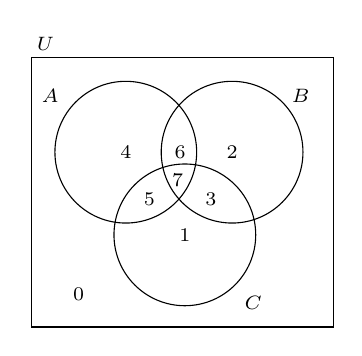
\begin{tikzpicture}[scale=0.6]
                \draw (-2,2) rectangle (4.4cm,-3.7cm);
                \draw (0,0) circle (1.5cm) node {};
                \draw (2.25,0) circle (1.5cm) node {};
                \draw (1.25,-1.75) circle (1.5cm) node {};
                \node at (0,0)  (a) {\scriptsize $4$};
                \node at (2.25,0)  (b) {\scriptsize $2$};
                \node at (1.25,-1.75)  (c) {\scriptsize $1$};
                \node at (1.8,-1)  (d) {\scriptsize $3$};
                \node at (1.15,0)  (e) {\scriptsize $6$};
                \node at (0.5,-1)  (f) {\scriptsize $5$};
                \node at (1.1,-0.6)  (e) {\scriptsize $7$};
                \node at (-1,-3)  (g) {\scriptsize $0$};
                \node at (-1.6,1.2) (h) {\scriptsize $A$};
                \node at (3.7,1.2) (i) {\scriptsize $B$};
                \node at (2.7,-3.2) (j) {\scriptsize $C$};
                \node at (-1.7,2.3) (k) {\scriptsize $U$};
            \end{tikzpicture}%}
        \end{minipage}%
        \begin{minipage}{10.5cm}
            Skup $A=\{4, 5, 6, 7\}$, skup $B=\{2, 3, 6, 7\}$ i skup $C=\{1, 3, 5, 7\}$.\\

            Skup $C\cup A=\{1, 3, 4, 5, 6, 7\}$, a skup $B\cup C=\{1, 2, 3, 5, 6, 7\}$.\\
            Dalje skup $(C\cup A)\setminus (B\cup C)=\{1, 3, 4, 5, 6, 7\}\setminus \{1, 2, 3, 5, 6, 7\}=\{4\}$.\\

            Na drugoj strani, skup $C\cup B=\{1, 2, 3, 5, 6, 7\}$.\\
            Pa skup $A\setminus (C\cup B)=\{4, 5, 6, 7\}\setminus \{1, 2, 3, 5, 6, 7\}=\{4\}$.\\

            Kako obje strane sadrže identična polja vennovog dijagrama, pokazali smo da su jednake tojest,
            $$(C\cup A)\setminus (B\cup C)=A\setminus (C\cup B)$$
        \end{minipage}
        \end{figure}
\end{dokaz}

\end{document} 